\newpage
\section{Continuous Learning}
\label{sec:continuous_learning}

Beim obigen Beispiel (Perceptron) wurde der Error berechnet indem der Vorhersagewert (Klasse, 1 oder 0) vom erwarteten Wert subtrahiert wurde.

In diesem Kapitel werden Ansätze angeschaut, welche auch schauen \textbf{wie weit weg} die Vorhersage war.

\subsection{Adaline}
%\begin{flushleft}

Adaline steht für \textbf{Adaptive Linear Neuron} und ist ein \textbf{supervised classification Algorithmus}. Adaline funktioniert wie folgt:

\begin{itemize}
  \item Die Elemente des Input-Vektors (Featurevektors) werden jeweils mit einem Gewicht multipliziert und aufsummiert.
  \item Die Summe (z) wird einer \textbf{Aktivierungsfunktion} übergeben, welche den Wert $\hat{y}$ erzeugt.
  \item $\hat{y}$ wird dann verwendet, um den \textbf{Fehler} bzw. das \textbf{Update für die Gewichte} zu berechnen.
  \item $\hat{y}$ wird zudem einer \textbf{Schwellwertfunktion} übergeben, welche die Features einer Klasse zuordnet.
\end{itemize}




\newcommand{\myThresholdFunction}{
\draw[thick] %(-2.25em,0em) -- (1.25em,0em) 
			 (-0.5em,1.25em) -- (-0.5em,-1.25em)
(-0.5em,1.25em) -- (0.5em,1.25em)
(-0.5em,-1.25em) -- (-1.5em,-1.25em)
;}


\begin{figure}[H]
\centering
\label{fig:perceptron}
\begin{tikzpicture}[
     % define styles 
     clear/.style={ 
         draw=none,
         fill=none
     },
     net/.style={
         matrix of nodes,
         nodes={ draw, circle, inner sep=10pt },
         nodes in empty cells,
         column sep=1.5cm,
         row sep=-9pt
     },
     >=latex
]
% define matrix mat to hold nodes
% using net as default style for cells
\matrix[net] (mat)
{
% Define layer headings
|[clear]| \parbox{1.3cm}{\centering Input\\layer} & 
|[clear]| \parbox{1.3cm}{\centering Gewichtete\\Summe} &
|[clear]| \parbox{1.3cm}{\centering Aktivierungs\\funktion} &
|[clear]| \parbox{1.3cm}{\centering Schwellwert\\Funktion} \\
         
$+1$  		& |[clear]| & Error     & |[clear]| \\
|[clear]| 	& |[clear]| & |[clear]| & |[clear]| \\
$x_{1}$  	& |[clear]| & |[clear]| & |[clear]| \\
|[clear]| 	& $\Sigma$  & $\phi$ & \myThresholdFunction \\
\vdots  	& |[clear]| & |[clear]| & |[clear]| \\
|[clear]| 	& |[clear]| & |[clear]| & |[clear]| \\
$x_{n}$  	& |[clear]| & |[clear]| & |[clear]| \\
};
\draw[->] (mat-2-1) -- node[above=1mm] {$w_{0}$} (mat-5-2);
\draw[->] (mat-4-1) -- node[above=1mm] {$w_{1}$} (mat-5-2);
\draw[->] (mat-6-1) -- node[above=1mm] {$\vdots$} (mat-5-2);
\draw[->] (mat-8-1) -- node[above=1mm] {$w_{n}$} (mat-5-2);
\draw[->] (mat-5-2) -- node[above=1mm] {$z$} (mat-5-3);
\draw[->] (mat-5-3) -- node[above=1mm] {$\hat{y}$} (mat-5-4);
\draw[->] (mat-5-3) -- node[above=1mm] {$$} (mat-2-3);
\draw[->] (mat-2-3) -- node[above=1mm] {Update Gewichte} (-2.5cm, 1cm);

\draw[->] (mat-5-4) -- node[right=2em] {$\begin{cases}
       		1 & \text{wenn } \hat{y} \geq 0, \\
       		0 & \text{sonst.}
    	\end{cases}$} +(2cm,0);
\end{tikzpicture}
\caption{Adaline als Model}
\label{fig:adaline_model}
\end{figure}


\newpage
Hier eine vereinfachte Beschreibung des Adaline-Models.

\textbf{Training} \\
Füge Bias-Gewicht (1) an Stelle Feature-0 hinzu.
Bestimme $z$:
\begin{align*}
	z &= w^{T} \times x \\
	z &= \sum_{i=0}^{n} w_{i}x_{i}  \\
\end{align*}


Einfachheitshalber nutzen wir für die \textbf{Aktivierungsfunktion} die Identitätsfunktion:
 $$\phi(z) = z$$
 
 Rechne nach jeder \textbf{Epoche} den Error aus und aktualisiere dementsprechend die Gewichte.



\textbf{Prediction} \\
Nun benötigen wir nur noch eine \textbf{Schwellwertfunktion} (decision function), die die vorhergesagte Klasse bestimmt.

$$ d(\hat{y}) =
\begin{cases}
	1 & \text{wenn } \hat{y} \geq 0, \\
	0 & \text{sonst.}
\end{cases}
$$


% ============================================
\newpage
\subsubsection{Adaline vs Perceptron}

Ähnlich wie der Perceptron ist Adaline ein Einzellayer neuronales Netzwerk. Der Hauptunterschied liegt auf der Aktivierungsfunktion phi $\phi(z)$


\begin{itemize}
  \item Der \textbf{Perceptron} aktualisiert die Gewichte nur, wenn eine falsche Vorhersage getroffen wurde. Zudem wird die Error-Funktion erst nach der \textbf{Schwellwertfunktion} aufgerufen. Somit wird ihr stets immer nur eine 0 oder 1 übergeben.
  \item \textbf{Adaline} hingegen aktualisiert die Gewichte basierend auf einer \textbf{stetigen} Funktion (continuous). Der \textbf{Aktivierungsfunktion $\phi$}
 \end{itemize}



Wie in Abbildung \ref{fig:adaline_vs_perceptron} ersichtlich ist, werden die Gewichte bei Adaline \textbf{vor} der Entscheidungsfunktion aktualisiert.

\begin{figure}[h!]
	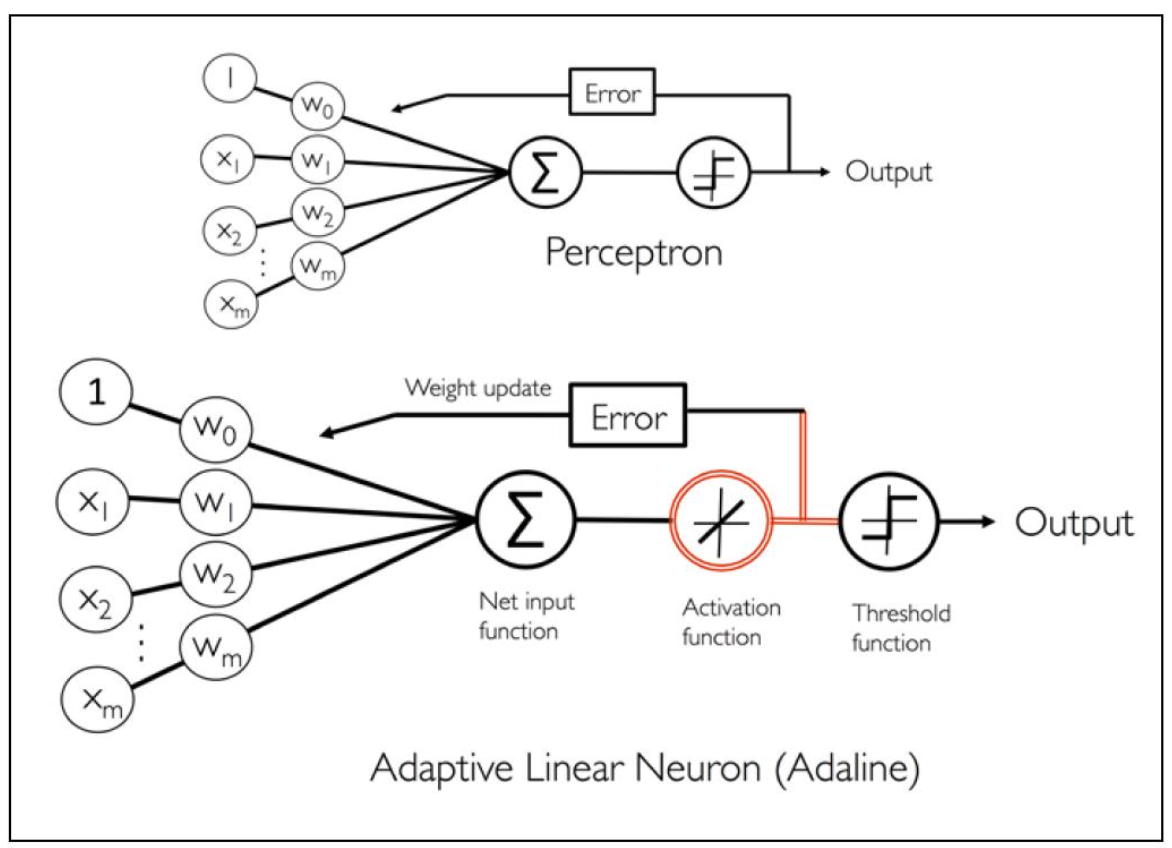
\includegraphics[scale=0.6]{figures/adaline_vs_perceptron}
	\caption{Adaline vs Perceptron}
	\label{fig:adaline_vs_perceptron}
\end{figure}

Im Gegensatz zum \textbf{binären Lernansatz} des Perceptron basieren viele supervised learning Algorithmen auf einer sogenannten \textbf{objective learning function}.


\newpage
\subsubsection{Objective Function}

Die Objective Function (Zielfunktion) ist mathematisch eine \textbf{Optimierung}.

Das Ziel hierbei ist es \textbf{optimale Parameter} zu finden. Optimal bedeutet den Output der Funktion entweder zu \textbf{maximieren} oder zu \textbf{minimieren}. 


Bei Machine Learning entsprechen die Parameter den \textbf{Gewichten}.


Eine Objective Funktion berechnet einen Output basierend auf den Eingaben:

\begin{itemize}
  \item Vorhersage (prediction)
  \item Eigentlicher Wert (labelled value)
\end{itemize}

Hierbei soll deren Differenz möglichst klein werden. Somit ist die Vorhersage sehr nahe am eigentlichen Wert. Ein Beispiel dafür zeigt Abbildung \ref{fig:objective_minimum}. 


\begin{figure}[h!]
	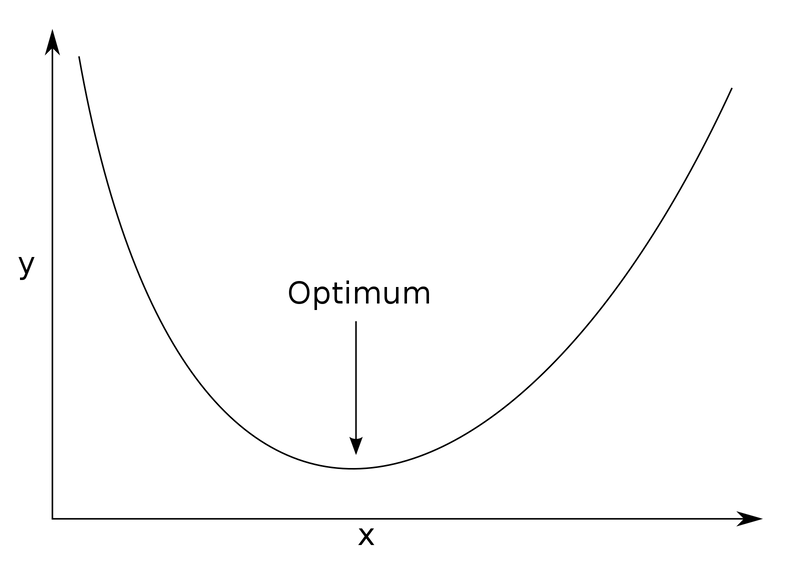
\includegraphics[scale=0.4]{figures/objective_minimum}
	\caption{Beispiel Zielfunktion}
	\label{fig:objective_minimum}
\end{figure}



Objective Funktion ist ein sehr genereller Term im Bereich ML.
Meistens wollen wir den Output der Objective Funktion \textbf{minimieren}. In diesem Fall sprechen wir von einer \textbf{Cost Function} oder \textbf{Loss Function}.


Wollen wir den Output \textbf{maximieren} so sprechen wir von einer \textbf{Likelihood Maximization} Funktion.



 
\newpage
\subsubsection{Objective Function in Adaline}

Adaline verwendet die Cost Function \textbf{Sum of Squared Errors (SSE)}.

SSE summiert alle quadrierten Differenzen zwischen Vorhersage und effektivem Wert auf.

$$ SSE = \frac{1}{2} \sum_{i=1}^{m}(y^{(i)} - \hat{y}^{(i)})^{2} $$

Hier eine detailliertere Darstellung von $\hat{y}$

$$ SSE = \frac{1}{2} \sum_{i=1}^{m}(y^{(i)} - \phi(z^{(i)}))^{2} $$


Wichtig zu wissen:
\begin{itemize}
  \item Die Funktion SSE ist \textbf{differenzierbar (ableitbar)}. Daher kann für jeden Punkt die Steigung berechnet werden.
  \item Sie hat ein \textbf{globales Minimum}.
\end{itemize}


Diese beiden Punkte sind notwendig für \textbf{Optimierungsalgorithmen}. Diese helfen dabei den Wert der Gewichte zu bestimmen damit die Cost Function möglichst klein wird. (Bsp. Gradient Descent)


\subsubsection{Adaline Learning Rule}

Die Gewicht-Updates werden anhand von \textbf{allen Samples} berechnet (Summe von 1 bin m). Daher werden die Gewichte auch immer erst nach einem vollen Trainingsdurchlauf aktualisiert und nicht nach jedem Sample.

Diese Art von Aktualisierung wird \textbf{batch gradient descent} genannt.

\begin{align*}
	\Delta w &= \eta \sum_{i=1}^{m} (y^{(i)} - \phi(z^{(i)}))^{2} * x^{(i)} \\
	w &= w + \Delta w \\
\end{align*}

\begin{align*}
	w &= \text{Gewichtsvektor} \\
	\Delta w &= \text{Gewichtsupdate (Vektor)} \\
	\eta &= \text{Learning Rate} \\
	m &= \text{Anzahl Samples}	\\
	y^{(i)} &= \text{Effektiver Zielwert (Label)} \\
	\phi &= \text{Aktivierungsfunktion} \\
	z^{(i)} &= \text{Summe der Input-Gewicht-Multiplikationen} \\
	x^{(i)} &= \text{Feature-Vektor des Samples i} \\
\end{align*}


\subsubsection{Adaline Optimierung mit Gradient Descent}

Für Adaline kann \textbf{Gradient Descent Algorithmus} zur Justierung verwendet werden.

Die Gewichtsupdates können nun so berechnet werden:

$$ \Delta w = - \eta \nabla J(w) $$

\begin{align*}
	J &= \text{Kostenfunktion (bspw. SSE)} \\
	\nabla &= \text{Symbol für Gradient (Steigung)} \\
	w &= \text{Gewichtsvektor} \\
\end{align*}


Wir berechnen also jeweils die \textbf{Steigung der cost function} am Punkt $P(w, J(w))$.

Der Gradient Descent wird in Kapitel \ref{sec:gradient_descent_basics} genauer erklärt.

% ==================================
\subsection{Gradient Descent Basics}
\label{sec:gradient_descent_basics}

Dieses Kapitel behandelt den Stoff zu Gradient Descent, welcher im Rahmen der Vorlesung behandelt wurde. Vertiefte Informationen zu Gradient descent sind Kapitel \ref{sec:gradient_descent} zu entnehmen.


\begin{itemize}
	\item Die \textbf{optimalen Gewichte} für eine \textbf{objective function} zu finden ist sehr rechenintensiv.
	\item Umso mehr Features vorhanden sind, desto mehr Gewichte hat unser Model.
	\item Daher auch mehr Kombinationen, wie die Gewichte gewählt werden könnten.
\end{itemize}

Optimisierungsalgorithmen (bspw. Gradient Descent) helfen dabei eine effiziente Lösung für die optimalen Gewichte zu finden.


\newpage
\subsubsection{Funktionsweise}

Abbildung \ref{fig:gradient_descent_simple} stellt eine vereinfachte Funktionsweise des GD dar.

\begin{itemize}
	\item Auf der y-Achse sind die Kosten (cost function)
	\item Auf der x-Achse sind die Gewichte. In diesem Beispiel haben wir nur ein Gewicht. Eigentlich wäre die Funktion aber multidimensional.
	\item Der schwarze Punkt zeigt die Ausgangslage bei zufällig initialisierten Gewichten.
	\item Der GD rechnet nun jeweils für die aktuelle Position $P(w, J(w))$ die Steigung aus.
	\item Ist die Steigung positiv müssen wir nach links gehen, um näher ans optimale Minimum zu gelangen. Also das Gewicht reduzieren.
	\item Ist die Steigung negativ, so gehen wir nach rechts indem wir das Gewicht erhöhen.
	\item Die Grösse der Schritte, die wir nach Links oder Rechts gehen wird von der \textbf{learning rate $\eta$} beeinflusst.
\end{itemize}

\begin{figure}[h!]
	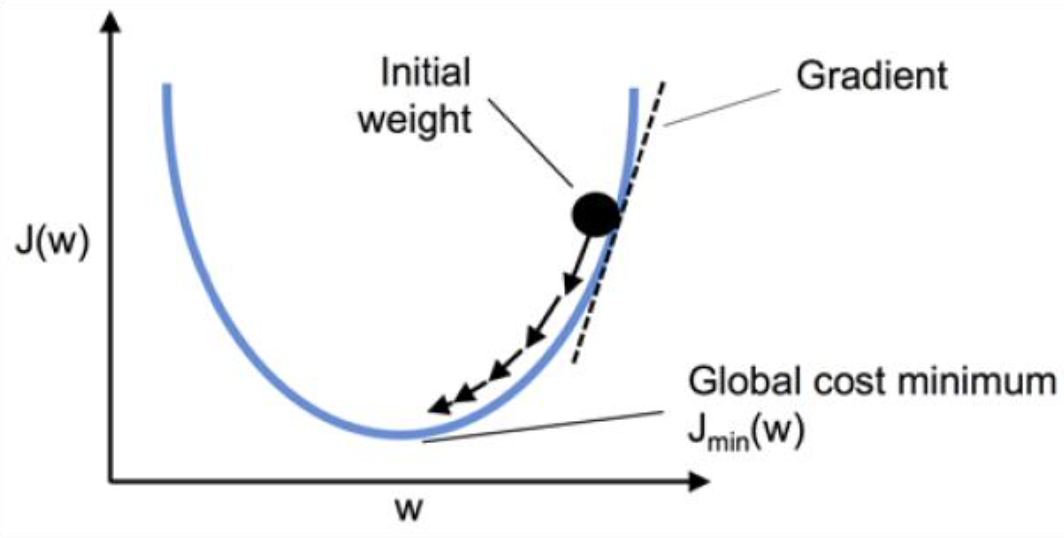
\includegraphics[scale=0.5]{figures/gradient_descent_simple}
	\caption{Gradient Descent Funktionsweise}
	\label{fig:gradient_descent_simple}
\end{figure}

Abbildung \ref{fig:gd_simple_multi} zeigt wie der GD bei mehreren Gewichten aussehen könnte.


\newpage
\subsubsection{Verhalten des GD}

Eine \textbf{optimale cost function ist konvex}. Also wie eine Schüssel geformt. Somit hat die Funktion nur \textbf{ein} Minimum. (Abbildung \ref{fig:gradient_descent_simple})


In der Praxis sehen die Funktionen aber meist wie
bspw. Abbildung \ref{fig:gd_simple_multi} aus. Diese Funktion hat ein \textbf{globales Minimum} und mehrere \textbf{lokale}. Das globale ist der optimale Wert unserer cost function. Doch nicht immer vom GD erreichbar.

\begin{figure}[h!]
	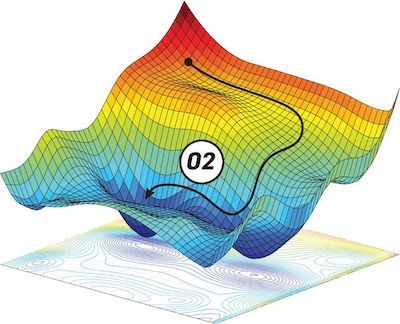
\includegraphics[scale=0.6]{figures/gd_simple_multi}
	\caption{Gradient Descent multidimensional}
	\label{fig:gd_simple_multi}
\end{figure}


\begin{itemize}
	\item Wird die \textbf{learning rate zu hoch} gewählt, ist es möglich, dass der GD stets \textbf{über} dem Minimum rüber springt.
	\item Ist sie \textbf{zu tief}, so könnte der GD in einem \textbf{lokalen Minumum} festsitzen.
\end{itemize}

\begin{figure}
    \centering
    \subfloat[]{{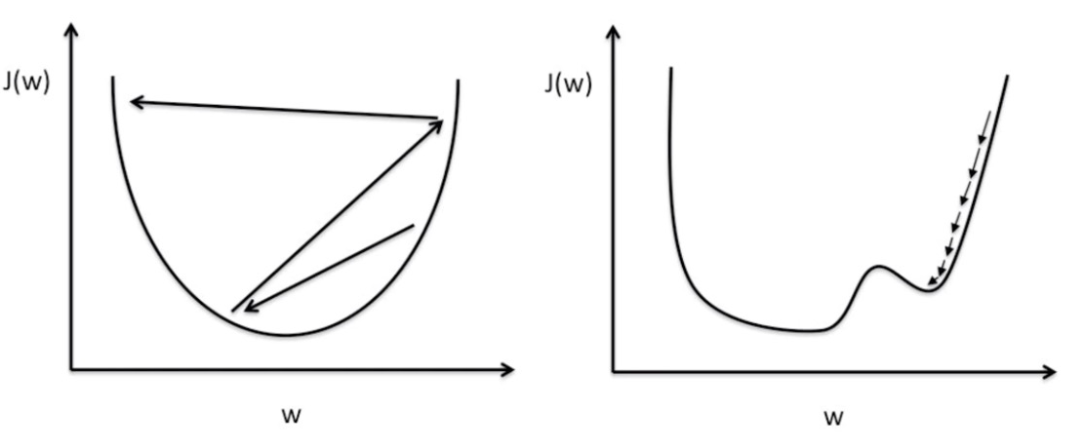
\includegraphics[scale=0.5]{figures/gd_behaviour} }}%
    \qquad
    \subfloat[]{{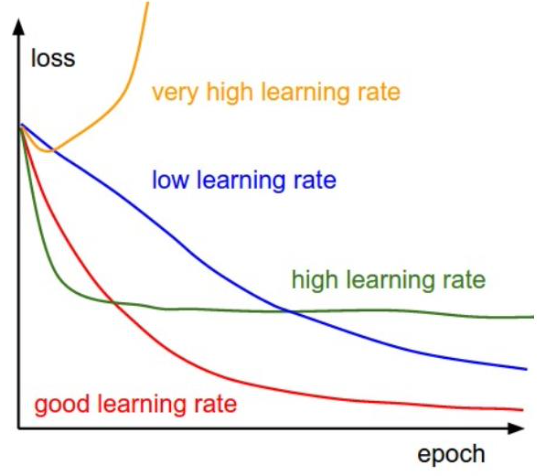
\includegraphics[scale=0.5]{figures/gd_learning_rate} }}%
    \caption{GD learning rate}%
    \label{fig:gd_learning_rate}%
\end{figure}


\newpage
\subsubsection{Arten von GD}

Es gibt verschiedene Möglichkeiten den Gradient Descent zu berechnen.

\textbf{Batch Gradient Descent (BGD)} \\


\begin{itemize}
	\item Verwendet \textbf{alle} Samples der Trainingsdaten \textbf{für eine einzige} Gewichtsaktualisierung.
	\item Für jedes Gewicht (bzw. Feature) wird der Error berechnet, indem der Durchschnittswert über alle Samples verwendet wird.
	\item Outliers haben weniger Einfluss auf die Gewichtsanpassung.
\end{itemize}

Dies führt zu einem stabilen Pfad hin zur Konvergenz gegen das Minimum. \\

Nachteile des BGD:

\begin{itemize}
	\item Schwierig zu \textbf{Skalieren}
	\begin{itemize}
		\item Alle Trainingsdaten (Matrix X) muss in RAM passen.
		\item Pro eine Gewichtsanpassung muss das ganze Trainingset einmal durchlaufen werden. Benötigt viel Epochen.
		\item Heutzutage nicht mehr ganz so tragisch.
	\end{itemize}
	\item Resultierendes Model hat Schwierigkeiten zu \textbf{generalisieren}
	\begin{itemize}
		\item Model leidet oftmals an \textbf{overfitting}
		\item Hauptgrund, um BGD nicht zu verwenden.
	\end{itemize}
\end{itemize}




\textbf{Stochastic Gradient Descent (SGD)} \\

Der stochastischen GD aktualisiert die Gewichte nach \textbf{jedem Schritt (nach jedem einzelnen Sample)}. Dies ist hilfreich für \textbf{grössere Mengen an Trainingsdaten}, da weniger Epochen ausgeführt werden müssen. SGD ist also 

\begin{itemize}
	\item Ist effizienter zu \textbf{Skalieren}
	\item Kleinere Tendenz für \textbf{overfitting} im Vergleich zu BGD.
\end{itemize}


Die Gewichte werden nach jedem Schritt wie folgt berechnet:
$$ w = w - \eta \nabla_{w} J(x^{(i)}, y^{(i)}, w) $$


Nachteile des SGD:

\begin{itemize}
	\item Benötigt viele Trainingsschritte
	\item Ausreisser können den SGD in eine falsche Richtung führen.
\end{itemize}


\newpage
\textbf{Mini-Batch Gradient Descent (MBGD)} \\

Wird oft verwendet. Ist ein \textbf{Kompromiss} zwischen BGD und SGD.
Das Gewichtsupdate wird anhand von $b$ vielen Samples berechnet.

$$ w = w - \eta \nabla_{w} J(x^{(i:i+b)}, y^{(i:i+b)}, w) $$ \\


\begin{itemize}
	\item Hilft \textbf{Overfitting / generalization error} zu vermeiden
	\begin{itemize}
		\item Die Batchgrösse $b$ muss wesentlich kleiner sein als die Anzahl Samples $m$.
		\item Dadurch wird dem Lernprozess \textbf{Noise} beigefügt.
	\end{itemize}
	\item Ist \textbf{schneller} als SGD
	\begin{itemize}
		\item Berechnungen erfolgen auf einer Matrix und nicht auf einzelnen Werten.
		\item Dies erlaubt effiziente Berechnungen mittels \textbf{Vektorisierung}.
	\end{itemize}
\end{itemize}


\textbf{Weitere Varianten} \\

\begin{itemize}
	\item AdaGrand (Adaptive Gradient Descent)
	\begin{itemize}
		\item Verschiedene learning rates für jedes Feature
		\item Nicht alle Features haben die gleichen \textbf{Seltenheit} (sparsity) und Werteverteilungen.
		\item Eine höhere learning rate für seltene (sparse) Features steigert deren Beitrag.
		\item Gut geeignet für NLP.
	\end{itemize}
	\item RMSprop
	\begin{itemize}
		\item Learning rate nimmt im Verlauf der Zeit ab.
		\item Umso kleiner die Steigung wird, desto kleiner wird die learning rate.
	\end{itemize}
\end{itemize}





